\documentclass[12pt]{article}
\usepackage[paper=letterpaper,margin=1.5cm]{geometry}
\usepackage{amsmath}
\usepackage{amssymb}
\usepackage{amsfonts}
\usepackage{mathtools}
%\usepackage[utf8]{inputenc}
%\usepackage{newtxtext, newtxmath}
\usepackage{lmodern}     % set math font to Latin modern math
\usepackage[T1]{fontenc}
\renewcommand\rmdefault{ptm}
%\usepackage{enumitem}
\usepackage[shortlabels]{enumitem}
\usepackage{titling}
\usepackage{graphicx}
\usepackage[colorlinks=true]{hyperref}
\usepackage{setspace}
\usepackage{subfigure} 
\usepackage{braket}
\usepackage{color}
\usepackage{tabularx}
\usepackage[table]{xcolor}
\usepackage{listings}
\usepackage{mathrsfs}
\usepackage{stackengine}
\usepackage{physics}
\usepackage{afterpage}
\usepackage{pdfpages}
\usepackage[export]{adjustbox}
\usepackage{biblatex}

\setstackEOL{\\}

\definecolor{dkgreen}{rgb}{0,0.6,0}
\definecolor{gray}{rgb}{0.5,0.5,0.5}
\definecolor{mauve}{rgb}{0.58,0,0.82}


\lstset{frame=tb,
  language=Python,
  aboveskip=3mm,
  belowskip=3mm,
  showstringspaces=false,
  columns=flexible,
  basicstyle={\small\ttfamily},
  numbers=none,
  numberstyle=\tiny\color{gray},
  keywordstyle=\color{blue},
  commentstyle=\color{dkgreen},
  stringstyle=\color{mauve},
  breaklines=true,
  breakatwhitespace=true,
  tabsize=3
}
\setlength{\droptitle}{-6em}

\makeatletter
% we use \prefix@<level> only if it is defined
\renewcommand{\@seccntformat}[1]{%
  \ifcsname prefix@#1\endcsname
    \csname prefix@#1\endcsname
  \else
    \csname the#1\endcsname\quad
  \fi}
% define \prefix@section
\newcommand\prefix@section{}
\newcommand{\prefix@subsection}{}
\newcommand{\prefix@subsubsection}{}
\renewcommand{\thesubsection}{\arabic{subsection}}
\makeatother
\DeclareMathOperator*{\argmin}{argmin}
\newcommand{\partbreak}{\begin{center}\rule{17.5cm}{2pt}\end{center}}
\newcommand{\alignbreak}{\begin{center}\rule{15cm}{1pt}\end{center}}
\newcommand{\tightalignbreak}{\vspace{-5mm}\alignbreak\vspace{-5mm}}
\newcommand{\hop}{\vspace{1mm}}
\newcommand{\jump}{\vspace{5mm}}
\newcommand{\R}{\mathbb{R}}
\newcommand{\C}{\mathbb{C}}
\newcommand{\N}{\mathbb{N}}
\newcommand{\G}{\mathbb{G}}
\renewcommand{\S}{\mathbb{S}}
\newcommand{\bt}{\textbf}
\newcommand{\xdot}{\dot{x}}
\renewcommand{\star}{^{*}}
\newcommand{\ydot}{\dot{y}}
\newcommand{\lm}{\mathrm{\lambda}}
\renewcommand{\th}{\theta}
\newcommand{\id}{\mathbb{I}}
\newcommand{\si}{\Sigma}
\newcommand{\Si}{\si}
\newcommand{\inv}{^{-1}}
\newcommand{\T}{^\intercal}
\renewcommand{\tr}{\text{tr}}
\newcommand{\ep}{\varepsilon}
\newcommand{\ph}{\varphi}
%\renewcomand{\norm}[1]{\left\lVert#1\right\rVert}
\definecolor{cit}{rgb}{0.05,0.2,0.45}
\addtolength{\jot}{1em}
\newcommand{\solution}[1]{

\noindent{\color{cit}\textbf{Solution:} #1}}

\newcounter{tmpctr}
\newcommand\fancyRoman[1]{%
  \setcounter{tmpctr}{#1}%
  \setbox0=\hbox{\kern0.3pt\textsf{\Roman{tmpctr}}}%
  \setstackgap{S}{-.9pt}%
  \Shortstack{\rule{\dimexpr\wd0+.1ex}{.9pt}\\\copy0\\
              \rule{\dimexpr\wd0+.1ex}{.9pt}}%
}

\newcommand{\Id}{\fancyRoman{2}}

% Enter the specific assignment number and topic of that assignment below, and replace "Your Name" with your actual name.
\title{STAT 30900: Homework 1}
\author{Caleb Derrickson}
\date{October 20, 2023}

\begin{document}
\onehalfspacing
\maketitle

{\color{cit}\vspace{2mm}\noindent\textbf{Collaborators:}} The TA's of the class, as well as Kevin Hefner, and Steven Lee.

\tableofcontents

\newpage
\section{Problem 1}

\subsection{Problem 1, part a} Let $A \in \C^{m \times n}$ and $1 \leq p \leq \infty$. Find the closed form expressions for 
\[
\lVert A \rVert_{1, p} := \max_{\textbf{x} \neq \textbf{0}} \frac{\lVert A\textbf{x} \rVert_{p}}{\lVert \textbf{x} \rVert_1} \hspace{5mm} \text{and} \hspace{5mm} \lVert A \rVert_{p, \infty} := \max_{\textbf{x} \neq \textbf{0}} \frac{\lVert A\textbf{x} \rVert_{\infty}}{\lVert \textbf{x} \rVert_p} 
\]
Your expressions should agree with the matrix 1-norm and matrix $\infty$-norm when $p = 1$ and $\infty$ respectively.
\partbreak
\begin{solution}

    Let $A_k$ denote the k-th column of $A$. Then, 
    \alignbreak
    \begin{align}
        \norm{A\textbf{x}}_p &= \norm{\sum_{k = 1}^n x_kA_k}_p &\text{(Definition of vector norm.)}\nonumber\\
        &\leq \sum_{k = 1}^n \norm{x_kA_k}_p &\text{(Triangle Inequality.)}\nonumber\\
        &= \sum_{k = 1}^n|x_k|\norm{A_k}_p &\text{(Absolute Homogeneity of norm.)}\nonumber\\
        &\leq \max \{ \norm{A_k}_p : 1 \leq k \leq n \} \Bigg(\sum_{k = 1}^n |x_k| \Bigg) &\text{(All columns of A are $\leq$ max column.)}\nonumber\\
        &=\max \{ \norm{A_k}_p : 1 \leq k \leq n \} \norm{\textbf{x}_1} &\text{(Definition of 1-norm.)}\nonumber\\
        \implies \frac{\norm{A\textbf{x}}_p}{\norm{\textbf{x}}_1} &\leq \max \{\norm{A_k}_p : 1 \leq k \leq n \} &\text{(Rearranging.)}\label{p1a:pnorm}
    \end{align}
    \alignbreak

    From \ref{p1a:pnorm}, this means the argument inside the max is less than or equal to the max column of $A$. The question now is when this is equal to $\norm{A}_{1,p}$. We are free to choose any nonzero \textbf{x}, so a natural one to choose would be the one to pick the max column when multiplied to $A$. Meaning if \textbf{x} $= e_M$, where M is the index corresponding to the max column of $A$, then equality it obtained. Note this is given as the definition of $\norm{A}_1$ when $p = 1$. 
\newpage
    We next wish to find a closed form expression for $\norm{A}_{p, \infty}$. It follows the same processes done in the previous section, with some slight modifications.

    \alignbreak
    \begin{align}
        \norm{A\textbf{x}}_\infty &= \max \{ |(A\textbf{x})_j | : 1 \leq j \leq n\} &\text{(Given.)}\nonumber\\
        &= \max \{ \Big|\sum_{k = 1}^nx_kA_{ik}\Big| : 1 \leq i \leq m\} &\text{(Matrix-vector multiplication.)}\nonumber\\
        &\leq \max \{ \sum_{k = 1}^n|x_kA_{ik}| : 1 \leq i \leq m\} &\text{(Triangle inequality.)}\nonumber\\
        &= \max \{ \sum_{k = 1}^n|x_k||A_{ik}| : 1 \leq i \leq m\} &\text{(Absolute Homogeneity.)}\nonumber\\
        &= \sum_{k = 1}^n|x_k||A_{Mk}| &\text{($M$ is max row of $A$.)}\nonumber\\
        &\leq |x_M|\sum_{k = 1}^n|A_{Mk}| &\text{($M$ is max element of \textbf{x}.)}\nonumber\\
        &= \norm{\textbf{x}}_\infty\sum_{k = 1}^n|A_{Mk}| &\text{(Definition of $\infty$-norm.)}\nonumber\\
        &\leq \norm{\textbf{x}}_p\sum_{k = 1}^n|A_{Mk}| &\text{($\infty$-norm is included in all $p$-norms.)}\nonumber\\
        \implies \norm{A\textbf{x}}_\infty &\leq \norm{\textbf{x}}_p\norm{A}_\infty &\text{(Definition of $\infty$-norm for matrices.)}\nonumber
    \end{align}
    \alignbreak

    Thus, we can see $\norm{A}_{p,\infty}$ is the max of $\norm{A}_\infty$, which is just $\norm{A}_\infty$. We note that $\norm{A}_\infty$ is the max row sum of the matrix $A$. Thus, both expressions have been found.
\end{solution}

\newpage
\subsection{Problem 1, part b}
Let $\S^n := \{ A \in \R^{n\times n} : A^T = A \}$. Recall the Gram matrix from Homework \textbf{0}, Problem \textbf{4}:
\\
For \textbf{x}$_1$, ..., \textbf{x}$_n \in \R^n$, we write

\[
G(\textbf{x}_1, ...,\textbf{x}_n) := 
\begin{bmatrix}
    \textbf{x}_1^T\textbf{x}_1 &\textbf{x}_1^T\textbf{x}_2 &... &\textbf{x}_1^T\textbf{x}_n\\
    \textbf{x}_2^T\textbf{x}_1 &\textbf{x}_2^T\textbf{x}_2 &... &\textbf{x}_2^T\textbf{x}_n\\
    \vdots    &\vdots     &\ddots    &\vdots\\
    \textbf{x}_n^T\textbf{x}_1 &\textbf{x}_n^T\textbf{x}_2 &... &\textbf{x}_n^T\textbf{x}_n\\
\end{bmatrix}
\in \S^n.
\]

Consider the set $\G^n := \{G(\textbf{x}_1, ..., \textbf{x}_n) \in \S^n : \norm{\textbf{x}_1}_2 \leq 1, ..., \norm{\textbf{x}_n}_2 \leq 1 \}$. Prove that for any $A \in \S^n$,

\[
\norm{A}_G := \max \{ |\text{tr}(AG)| : G \in \G^n \}
\]

defines a norm on $S^n$. Show that if $A$ = diag($a_{11}, ..., a_{nn}$) $\in \S^n$, then 
\[
\norm{A}_G = \max\bigg( \sum_{i = 1}^n \max (a_{ii}, 0), -\sum_{i = 1}^n \min (a_{ii}, 0)\bigg).
\]

\partbreak
\begin{solution}

    As A quick reminder, a norm $\norm{\cdot}$ should satisfy the following properties for scalar $\alpha$ and matrices $A, B \in \R^{n\times n}$:
    \jump
    \hrule
    \begin{enumerate}[(1)]
        \item $\norm{A} \geq 0$.
        \item $\norm{A} = 0 \iff A = 0$.
        \item $\norm{\alpha A} = |\alpha| \norm{A}$.
        \item $\norm{A + B} \leq \norm{A} + \norm{B}$.
    \end{enumerate}
    \hrule
    \jump
    Note that I'm taking $A, B \in \R^{n\times n}$ since the set $\S^n \subset \R^{n\times n}$. We will prove each property below.

    \begin{enumerate}[(1)]
        \item $\norm{A} \geq 0$.

        By the definition of $\norm{A}_G$, we are taking the maximum over a set of strictly positive elements - the absolute value guarantees this. Thus this property is immediately obeyed.

        \jump
        \item $\norm{A} = 0 \iff A = 0$.

        The backward implication is straightforward, as if $A = 0$, the $AG = 0$, thus the trace is taken over the zero matrix, meaning we are taking the maximum over the set containing only zeros, thus $\norm{A}_G = 0$.

        The forward implication requires jumping through some extra hoops. We can note that by the symmetry of the inner product of the real numbers, $G$ is symmetric for all $G \in \G^n$. 

            
    \end{enumerate}
\end{solution}
\newpage
\section{Problem 2}
Let $A \in \C^{n\times n}$ and $\lVert \cdot \rVert_p : \C^{n \times n} \rightarrow [0, \infty )$ be the matrix $p$-norm for some $p \in [1, \infty]$. 

\subsection{Problem 2, part a}
Show that if $\norm{A}_p < 1$, then $\Id - A$ is invertible and furthermore, 
\begin{align}
\frac{1}{1 + \lVert A\rVert_p} \leq \lVert(\Id - A)^{-1}\rVert_p \leq \frac{1}{1 - \lVert A\rVert_p}. \label{p2a:chain ineq}    
\end{align}
\partbreak
\begin{solution}

    Let \textbf{v} $\in \C^{n\times n} \backslash \{0\}$ be an eigenvector of $A$ with eigenvalue $\lm$. Then $A\textbf{v} = \lm \textbf{v} \iff \norm{A\textbf{v}}_p = \norm{\lm\textbf{v}}_p$. Note the matrix $p$-norm is taken as a max over all \textbf{x} $\neq 0$. Along with $\norm{A} < 1$, we get, 
    \[
    1 > \max_{\textbf{x} \neq 0}\frac{\norm{A\textbf{x}}}{\norm{\textbf{x}}} \leq \frac{\norm{A\textbf{v}}}{\norm{\textbf{v}}}
    \]
    then $\norm{A\textbf{v}} < \norm{\textbf{v}}$. So 1 is then not an eigenvector of $A$. This implies that $(A - \id)\textbf{v} = (\lm - 1)\textbf{v}$. Note that \textbf{v} was taken as a nonzero vector, so $(1 - \lm)\textbf{v} \neq 0$. This means that 0 is not an eigenvalue of $A - \id$, making the determinant nonzero, thus $A - \id$ is invertible.  

    \jump
    We then wish to show \ref{p2a:chain ineq},
    
    \[
    \frac{1}{1 + \lVert A\rVert_p} \leq \lVert(\Id - A)^{-1}\rVert_p \leq \frac{1}{1 - \lVert A\rVert_p}.
    \]
    
    \jump
    To prove the first inequality, we note that if \textbf{v} is an eigenvector of $A$ with eigenvalue $\lm$, (and $A$ invertible) then \textbf{v} is an eigenvector of $A$ with eigenvalue $\lm^{-1}$. This is shown by the following:
    
    \[
    A\textbf{v} = \lm\textbf{v} \iff A^{-1}A\textbf{v} = A^{-1}\lm\textbf{v} \iff A^{-1}\textbf{v} = \frac{1}{\lm} \textbf{v}.
    \]

    Thus, take \textbf{v} as an eigenvector of $A$ with eigenvalue $(1 - \lm)$. The above claim implies that \textbf{v} is also an eigenvector of $(\id - A)^{-1}$ with eigenvalue $(1 - \lm)^{-1}$. Furthermore, since $\norm{\cdot}_p$ is consistent, we have that the spectral radius $\rho(A) = \max\{ |\lm(A)|\}$ is less than or equal to $\norm{A}$, ie $\rho(A) \leq \norm{A}$. The following steps can then be justified

    \alignbreak
    \begin{align}
        &(\id - A)^{-1}\textbf{v} = \frac{1}{1 - |\lm|}\textbf{v}   &\text{(Given.)}\nonumber\\
        &\norm{(\id - A)^{-1}\textbf{v}} = \frac{1}{1 - |\lm|}\norm{\textbf{v}} &\text{(Taking norm and eigenvalue is positive.)}\nonumber\\
        &\norm{(\id - A)^{-1}\textbf{v}} \leq \norm{(\id - A)^{-1}}\norm{\textbf{v}}    &\text{(Norm Consistency of $\norm{\cdot}_p$.)} \label{p2a:normconsistency}\\
        \implies &\norm{(\id - A)^{-1}} > \frac{1}{1 - |\lm |} &\text{(Applying \ref{p2a:normconsistency} and cancelling $\norm{v}$)}\nonumber\\
        &\norm{(\id - A)^{-1}} > \frac{1}{1 + |\lm |} &\text{($1 - |\lm | < 1 + |\lm |$.)} \nonumber\\
        &\norm{(\id - A)^{-1}} \geq \frac{1}{1 + \norm{A}_p} &\text{($\rho(A) \leq \norm{A}$.)}\nonumber
    \end{align}
    \alignbreak

    This solves the first inequality of \ref{p2a:chain ineq}. We then can show the second inequality via the Taylor expansion of $\norm{(\id - A)^{-1}}_p$. Noting further that $\norm{A}_p < 1$, the following steps can be taken:

    \alignbreak
    \begin{align}
        &\norm{(\id - A)^{-1}}_p &\text{(Given.)}\nonumber\\
        &= \norm{\sum_{k = 0}^\infty A^k}_p &\text{(Taylor Expansion.)}\nonumber\\
        &\leq \sum_{k = 0}^\infty \norm{A^k}_p &\text{(Triangle inequality.)}\nonumber\\
        &\leq\sum_{k = 0}^\infty\norm{A}^k_p &\text{(Submultiplication of $\norm{\cdot}_p$.)}\nonumber\\
        \implies \norm{(\id - A)^{-1}}_p&\leq \frac{1}{1 - \norm{A}_p} &\text{(Taylor Expansion Equivalent.)}\nonumber
    \end{align}
    \alignbreak

    This proves both inequalities, thus \ref{p2a:chain ineq} has been shown. $\square$
\end{solution}

\subsection{Problem 2, part b}
Suppose $A$ is invertible. show that and $X \in \C^{n\times n}$ with
\[
\norm{X - A}_p < \frac{1}{\norm{A^{-1}}_p}
\]
must also be invertible. 
\partbreak

\begin{solution}

    We first should note that if a matrix product $AB$ is invertible, then both $A$ and $B$ are invertible. This can be reasoned by a rank argument: if $AB$ is invertible, then $AB$ has full rank. If $B$ mapped anything other than \textbf{0} to \textbf{0}, then $AB$ would map a nonzero vector to zero, which is a contradiction. Thus, $B$ has full rank, meaning that any vector in its target space can be represented by an element in the domain of $B$ scaled by matrix $B$ (i.e. $B\textbf{x} = \textbf{y}$). If we supposed that $A$ mapped $\textbf{y}$ to the zero vector for some arbitrary $\textbf{y}$, then $AB$ would map $\textbf{y}$ to zero, which can only be the zero vector. Thus $\textbf{y} = \textbf{0}$, meaning $A$ and $B$ have full rank, thus both are invertible. This will be used in the following steps:
    
    \alignbreak
    \begin{align}
        &\norm{X - A}_p < \frac{1}{\norm{A^{-1}}_p} &\text{(Given.)}\nonumber\\
        &\norm{X - A}_p\norm{A^{-1}}_p < 1  &\text{(Rearranging.)}\nonumber\\
        &\norm{(X - A)A^{-1}}_p \leq \norm{X - A}_p\norm{A^{-1}}_p &\text{(Norm submultiplicative.)}\label{p2b:normconsistency}\\
        \implies &\norm{XA^{-1} - AA^{-1}}_p < 1 &\text{(Applying \ref{p2b:normconsistency}.)}\nonumber\\
        &\norm{XA^{-1} - \id}_p < 1 &\text{(Simplifying.)}\nonumber\\
        \implies &\id - XA^{-1} + \id \text{ is invertible.} &\text{(By part a.)}\nonumber\\
        \implies &XA^{-1} \text{ is invertible.} &\text{(Simplifying.)}\nonumber\\
        \implies &X \text{ is invertible.} &\text{(By proof above.)}\nonumber
    \end{align}
    \alignbreak
    
    The steps above thus prove $X$ is invertible. $\square$
\end{solution}

\subsection{Problem 2, part c}
Let $\norm{\cdot} : \C^{n\times n} \rightarrow [0, \infty)$ be an arbitrary norm that may not be submultiplicative. Suppose $\norm{A} < 1$, can we conclude that $\id - A$ is invertible?
\partbreak

\begin{solution}

    As a counterexample, take A to be
    \[
    A = 
    \begin{bmatrix}
    1/2     &-1/2   \\
    -1/2    &1/2
    \end{bmatrix}
    \]

    Under the H\"{o}lder $\infty$-norm. Thus $\norm{A} < 1$, but 
    \[
    \id - A = 
    \begin{bmatrix}
    1/2     &1/2   \\
    1/2    &1/2
    \end{bmatrix}
    \]

    which is clearly not invertible, since $\id - A$ does not have full rank.
\end{solution}

\newpage
\section{Problem 3}
Recall that in the lectures, we mentioned that
\begin{enumerate}[(i)]
    \item there are matrix norms that are not submutiplicative and an example is the H\"{o}lder $\infty$-norm;
    \item we may always construct a norm that approximates the spectral radius of a given matrix $A$ as closely as we want.  
\end{enumerate}

\subsection{Problem 3, part a}
Let $\norm{\cdot} : \C^{m\times n} \rightarrow \R$ be a norm, defined for all $m, n \in \N$. show that there always exist a $c > 0$ such that the constant multiple $\norm{\cdot}_c := c\norm{\cdot}$ defines a submultiplicative norm, i.e.,
\[
\norm{AB}_c \leq \norm{A}_c\norm{B}_c
\]
for any $A \in \C^{m\times n}$ and $B \in \C^{n\times p}$ (even if $\norm{\cdot}$ does not have this property). Note that the constant $c$ will depend on $m, n, p \in \N$ in general. Find the constant $c$ for the H\"{o}lder $\infty$-norm. 

\partbreak
\begin{solution}

    By the Equivalence of Norms over a Finite Dimensional Vector Space, (in this case, $\C^{m\times n}$) there will exist some $0< a_1 < a_2$ such that 

\begin{align}
     a_1\norm{C}_* \leq \norm{C} \leq a_2\norm{C}_* \label{p3a: equiv}
\end{align}

for any norm $\norm{\cdot}_*$ over our space and matrix $C$. Consider the Frobenius norm, $\norm{\cdot}_F$. We know that the Frobenius norm obeys submultiplicivity, so the following steps are justified:

\alignbreak
\begin{align}
    \norm{AB} &\leq a_2\norm{AB}_F   &\text{(Equivalence.)}\nonumber\\
    &\leq a_2\norm{A}_F\norm{B}_F    &\text{(Submultiplicivity of F.)}\nonumber\\
    &\leq \frac{a_2}{a_1}\norm{A}\frac{1}{a_1}\norm{B}  &\text{(Equivalence.)}\nonumber\\
    &= \frac{a_2}{a_1^2}\norm{A}\norm{B}    &\text{(Rewriting.)}\nonumber
\end{align}
\alignbreak

Therefore, let $c = \frac{a_2}{a_1^2} > 0$. Thus $\norm{AB}_c \leq \norm{A}_c\norm{B}_c$.


We next wish to find the constant $c$ for the H\"{o}lder $\infty$-norm. We will be looking at its equivalence to the Frobenius norm. 

\alignbreak
\begin{align}
    \norm{AB}^2_F &= \sum_{i = 1}^m\sum_{j = 1}^p\Big|\sum_{k = 1}^nA_{ik}B_{kj}\Big|^2
    &\text{(Finding left inequality.)}\nonumber\\
    &\leq \sum_{i = 1}^mp\max_j \Big\{ \Big|\sum_{k = 1}^n A_{ik}B_{kj}\Big|^2\Big\}    &\text{(Taking max over B's columns.)}\nonumber\\
    &\leq mp\max_{ij}\Big\{ \Big| \sum_{k = 1}^nA_{ik}B_{kj}\Big|^2\Big\}   &\text{(Taking max over A's rows.)}\nonumber\\
    \implies \norm{AB}_F &\leq \sqrt{mp}\max_{ij}\Big\{\Big| \sum_{k = 1}^n A_{ik}B_{kj}\Big|\Big\} &\text{(Square root function is monotonic.)}\nonumber\\
    \iff \norm{AB}_F &\leq \sqrt{mp}\norm{AB}_{H, \infty}\label{p3a: left ineq}\\
    \norm{AB}^2_{H, \infty} &= \max_{ij}\Big\{\Big| \sum_{k = 1}^n A_{ik}B_{kj}\Big|\Big\} &\text{(Finding right inequality.)}\nonumber\\
    &\leq \max_{i}\Big\{\sum_{j = 1}^p\Big| \sum_{k = 1}^n A_{ik}B_{kj}\Big|\Big\} &\text{(Max over j is one of the sums.)}\nonumber\\
    &\leq \sum_{i = 1}^m\sum_{j = 1}^p\Big| \sum_{k = 1}^n A_{ik}B_{kj}\Big| &\text{(Same argument.)}\nonumber\\
    \implies \norm{AB}^2_{H, \infty} &\leq \norm{AB}_2^2 &\text{(Definition of Frobenius norm.)}\nonumber\\
    \iff \norm{AB}_{H, \infty} &\leq \norm{AB}_2\label{p3a: right ineq}
\end{align}

\alignbreak

In our calculations above, we can find values for $a_1, a_2$. Taking the factors in front of each norm, we get $a_1 = (\sqrt{mn})^{-1}$ and $a_2 = 1$. Note that these are not unique, since another valid value for $a_2$ is 2. It is entirely possible there could be smaller bounds which we could argue. These are just values I've found to work.  Thus $c$ will take the value $(mn)^{-1}$.

\newpage
\subsection{Problem 3, part b}
Let $J \in \C^{n\times n}$ be in Jordan form. Let $\ep > 0$. Verify that $D^{-1}_\ep J D_\ep$ replaces the ones along the superdiagonal by $1, \ep, \ep^2, ..., \ep^{n - 1}$.
\partbreak

Note for any Jordan matrix $J$ can be rewritten as a diagonal matrix $A$ plus a nilpotent matrix $N$ of some degree. I.e., $J = A + N$, where $N$ has value 1 only along the superdiagonal (hence N had nilpotency degree n). Therefore, we can rewrite $D^{-1}_\ep J D_\ep$ as the following:

\jump
\[
D^{-1}_\ep J D_\ep = D^{-1}_\ep (A + N) D_\ep = D^{-1}_\ep A D_\ep + D^{-1}_\ep N D_\ep
\]
\jump

Note that $D_\ep^{-1} = $ diag($ 1, \ep^{-1}, \ep^{-2}, ... \ep^{1 - n}$). Since A is diagonal, each column will be multiplied then divided by the same degree of $\ep$, i.e. column 1 of $A$ will be multiplied by $\ep^0$ then divided by $\ep^0$, column 2 of $A$ will be multiplied by $\ep^1$ then divided by $\ep^1$, and so on, doing nothing in the process. So $D^{-1}_\ep A D_\ep = A$. We just need to show that the nilpotent matrix $N$ will be multiplied by $\ep$.

\jump
Denote $\gamma_i$ as the $i$-th row of $D_\ep$, and $\eta_j$ as the $j$-th column of $N$. Note $N, D_\ep \in \C^{n\times n}$. So $i,j \leq n$; $\eta_j = e_{j + 1}$ for $j \neq 1$ and $\eta_1 = 0$; and $\gamma_i$ = $\ep^{i -1}e_i$, where $e_i$ is the $i$-th canonical basis vector. The following steps are then justified.

\alignbreak
\begin{align}
    ND_\ep &= \sum_{i = 1}^n \eta_i\gamma_i^t &\text{(Matrix product interpretation.)}\nonumber\\
    &= \sum_{i = 1}^n e_{i + 1}\ep^{i - 1}e_i^t &\text{(Plugging in).}\nonumber\\
    &= \text{superdiag}(\ep^2, \ep^3, ..., \ep^{n - 1}) &\text{(superdiag is shorthand.)}\nonumber
\end{align}
\alignbreak

I couldn't express the outer product $e_{i + 1}e_i^t$ elegantly, so please mind my shorthand notation of superdiag(-). The important thing to note here is that by our construction of $\eta_i$, the column of $D_\ep$ containing the linear $\ep$ is terminated, leaving us with the leading term being quadratic, $\ep^2$. We will then multiply on the left by $D_\ep^{-1}$ in a similar manner.

\newpage
\alignbreak
\begin{align}
    D^{-1}_\ep ND_\ep &= \sum_{i = 1}^n \ep^{1-i}e_i(ND_\ep)_i^t &\text{(Matrix product interpretation.)}\nonumber\\   
    &= \sum_{i = 1}^n \ep^{1-i}e_i\ep^ie_{i + 1}^t &\text{(Plugging in.)}\nonumber\\
    &= \sum_{i = 1}^n \ep^{1}(e_{i+1}^t)^*(e_i)^* &\text{(Antisymmetry of inner product.)}\nonumber\\
    &= \sum_{i = 1}^n \ep e_{i+1}e_i^t &\text{(Basis vectors are real.)}\nonumber\\
    D^{-1}_\ep ND_\ep &= \text{superdiag}(\ep, \ep, ..., \ep) &\text{(Shorthand.)}\nonumber
\end{align}
\alignbreak

Therefore we have proven the claim. 
\end{solution}

\subsection{Problem 3, part c}
Show that 
\[ 
\norm{D_\ep^{-1}JD_\ep}_\infty \leq \rho(J) + \ep
\]

\partbreak
\begin{solution}
    
It was shown in part b that the left and right multiplications of $D_\ep$ and its inverse did nothing to the diagonal of $J$. Since $J$ is an upper triangular matrix, its eigenvalues are located along its diagonal. Thus $\rho(J) = |\lm_M|$ for some $1 \leq M \leq k$. Note it could be the case that all eigenvalues are negative, thus when taking the $\infty$-norm, a different eigenvalue could be taken. Suppose $m$ is chosen such that $\norm{D_\ep^{-1}JD_\ep}_\infty = |\lm_m + \ep|$. By the triangle inequality, $|\lm_m + \ep| \leq |\lm_m| + \ep$, since $\ep$ is positive. But $|\lm_m| \leq \max_{i \leq k}\{|\lm_i|\} = \rho(J)$, thus $\norm{D_\ep^{-1}JD_\ep}_\infty \leq \rho(J) + \ep$. 
\end{solution}

\newpage
\subsection{Problem 3, part d}
Hence, or otherwise, show that for any given $A\in \C^{n\times n}$ and $\ep > 0$, there exists a norm $\norm{\cdot}_*$ on $\C^n$ such that 
\[
\norm{A} = \max_{\textbf{x} \neq \textbf{0}} \frac{\norm{A\textbf{x}}_*}{\norm{\textbf{x}}_*}
\]

has the property that 
\[
\rho(A) \leq \norm{A} \leq \rho(A) + \ep
\]
\partbreak

\begin{solution}
    
\end{solution}
\newpage
\section{Problem 4}
\textbf{Note that for simplicity I will provide the results before the code block(s).}

Let $A = [a_{ij}]$ be an $n \times n$ matrix with entries
\[
a_{ij} = 
\begin{cases}
    n + 1 - \max (i, j) &i \leq j + 1, \\
    0   & i > j + 1
\end{cases}
\]
This is an example of an \textit{upper Hessenberg} matrix: it is upper triangular except the entries on the subdiagonal $a_{j + 1, j}$ may also be non-zero. For $n = 12$ and $n = 25$, do the following:

\subsection{Problem 4, part a}
Compute $\norm{A}_\infty$ and $\norm{A}_1$.
\partbreak
\begin{solution}

    The methods to compute the 1-norm and $\infty$-norm are provided below, as well as the method to compute the Hessenberg matrix. The code which uses these functions are provided in the second block. . When running the code below, I get the following:
    \begin{itemize}
        \item Size 12 Hessenberg matrix: 1-norm: 55.0, inf-norm: 90.0
        \item Size 25 Hessenberg matrix: 1-norm: 195.0, inf-norm: 350.0
    \end{itemize}
    
\begin{lstlisting}
#Methods block
def compute_hessenberg_matrix(n):
    """
    Returns the Hessenberg matrix of given size
    """
    A = np.empty((n, n))
    for i in range(n):
        for j in range(n):
            if i <= j + 1:
                A[i][j] = n + 1 - max(i,j)
            else:
                A[i][j] = 0
    return A

def compute_inf_norm(A):
    """
    Returns the infinity norm of the given matrix 
    """
    row_sums = []
    for i in range(A.shape[0]):
        row_sum = 0
        for j in range(A.shape[0]):
            row_sum += abs(A[i][j])
        row_sums.append(row_sum)
    
    return max(row_sums)

def compute_1_norm(A):
    """"
    Returns the 1-norm of the given matrix
    """
    column_sums = []
    for i in range(A.shape[0]):
        column_sum = 0
        for j in range(A.shape[0]):
            column_sum += abs(A[j][i])
        column_sums.append(column_sum)
    
    return max(column_sums)

\end{lstlisting}
\begin{lstlisting}
#"Main"
hessenberg = [compute_hessenberg_matrix(x) for x in [12,25]]

#Computing the matrix inf and 1 norms for matrices
for matrix in hessenberg:
    print("Size {} Hessenberg matrix: 1-norm: {}, inf-norm: {}".format(matrix.shape[0], compute_1_norm(matrix), compute_inf_norm(matrix)))
\end{lstlisting}
\end{solution}

\newpage
\subsection{Problem 4, part b}
Compute $\rho(A)$ and $\norm{A}_2$. You may use any built-in functions of your program.
\partbreak
\begin{solution}

    The code I used to calculate this is given below. The result when running this block is given as 
    \begin{itemize}
        \item Size 12 \\
            Spectral Radius: 35.61 \\
            Matrix 2-norm 54.92 \\
        
        \item Size 25 \\
            Spectral Radius: 81.61 \\
            Matrix 2-norm 194.43
    \end{itemize}

\begin{lstlisting}
#Computing the spectral radius and 2-norm
for matrix in hessenberg:
    eigenvals = [x for x in abs(np.linalg.eigvals(matrix))]
    print("Size {} ".format(matrix.shape[0]))
    print("Spectral Radius: {:.2f}".format(max(eigenvals)))
    print("Matrix 2-norm {:.2f}".format(np.linalg.norm(matrix, ord=2)))
\end{lstlisting}
\end{solution}

\subsection{Problem 4, part c}
Using Gerschgorin’s theorem, describe the domain that contains all of the eigenvalues.

\partbreak
\begin{solution}
    The order of code shown will be given as: methods used, block to implement methods, then plotting. The resulting plots are given below. It seems that the radius of the balls increase with eigenvalue, resulting in the largest eigenvalue enclosing all smaller eigenvalues. I couldn't get the color bar to work exactly as I wanted, so just trust me on this.  

\vspace{\floatsep}
\clearpage

\jump
\begin{figure}[!ht]
\centering
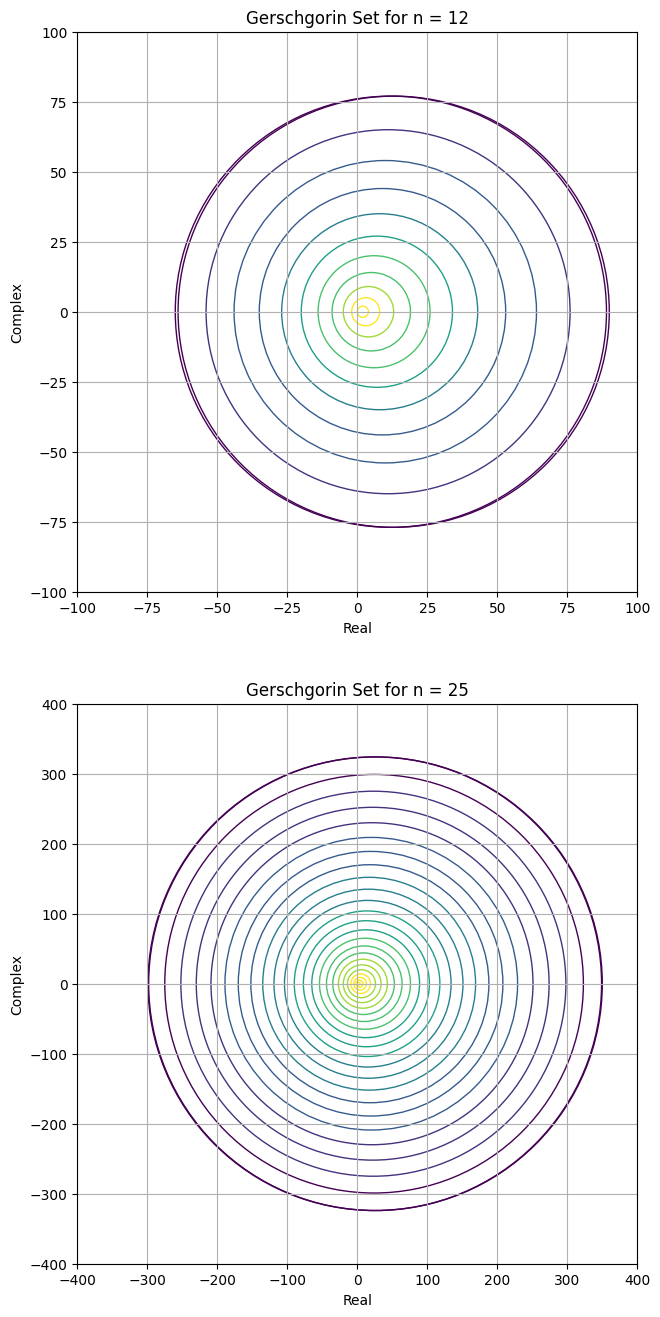
\includegraphics[scale = 0.6]{Images/gerschgorin balls.png}
\caption{Gerschgorin sets for Gessenberg matrices of n = 12, 25. Larger values $\rightarrow$ darker colors. }
\label{png:gerschgorin sets}
\end{figure}

\begin{lstlisting}
#Methods Block
def compute_gerschgorin_radius(row, diag_entry):
"""
Returns the summed absolute values of entries in the given row, 
minus the specified entry index
"""
row_sum = 0
for i in range(len(row)):
    if i != diag_entry:
        row_sum += abs(row[i])
        
return row_sum
\end{lstlisting}

\begin{lstlisting}
#Computing tuples containing the diagonal entry and its radius for Gerschgorin's Theorem

gerschgorin_balls = []
for matrix in hessenberg:
matrix_balls = []
for i in range(matrix.shape[0]):
    matrix_balls.append((matrix[i][i], compute_gerschgorin_radius(matrix[i], i)))
    gerschgorin_balls.append(matrix_balls)
\end{lstlisting}

\begin{lstlisting}
#Plotting block
#Setting Color scale
#Larger values -> darker colors
viridis = mpl.colormaps['viridis'].resampled(8)
color12 = viridis(np.linspace(0, 1, 12))
color25 = viridis(np.linspace(0, 1, 25))

fig, ax = plt.subplots(2, figsize=(24,16))

#Plotting the gerschgorin plot for n = 12
i = 0
for tup in gerschgorin_balls[0]:
    center = (tup[0], 0)
    circle = Circle(center, tup[1], fill=False, color=color12[i])
    ax[0].add_patch(circle)
    i +=1

ax[0].set_title("Gerschgorin Set for n = 12")
ax[0].set_aspect('equal', adjustable='box')
ax[0].set_xlim(-100, 100)
ax[0].set_xlabel("Real")
ax[0].set_ylim(-100, 100)
ax[0].set_ylabel("Complex")
ax[0].grid(True)  

#Plotting the gerschgorin plot for n = 25
i = 0
for tup in gerschgorin_balls[1]:
    center = (tup[0], 0)
    circle = Circle(center, tup[1], fill=False, color=color25[i])
    ax[1].add_patch(circle)
    i+=1
    
ax[1].set_title("Gerschgorin Set for n = 25")
ax[1].set_aspect('equal', adjustable='box')
ax[1].set_xlim(-400, 400)
ax[1].set_xlabel("Real")
ax[1].set_ylim(-400, 400)
ax[1].set_ylabel("Complex")
ax[1].grid(True)  
plt.show()
\end{lstlisting}
\end{solution}

\subsection{Problem 4, part d}
Compute all of the eigenvalues and singular values of $A$. How many of the eigenvalues are real and how many are complex? You may use any built-in functions of your program.
\partbreak
\begin{solution}

    The code I used to calculate this is shown below. The results from this code block is given as:
\begin{itemize}
    \item Size 12\\
          Real Eigenvalues: 12, Complex Eigenvalues: 0\\
          Real Singular: 12, Complex Singular: 0\\
    \item Size 25\\
          Real Eigenvalues: 13, Complex Eigenvalues: 12\\
          Real Singular: 25, Complex Singular: 0
\end{itemize}
    \begin{lstlisting}
for matrix in hessenberg:
    eigenvals = np.linalg.eigvals(matrix)
    real_eigenvals = 0
    complex_eigenvals = 0
    for val in eigenvals:
        if isinstance(val, complex):
            if val.imag != 0:
                complex_eigenvals+=1
            else:
                real_eigenvals+=1
        else:
            real_eigenvals+=1;
    
    real_sing = 0
    complex_sing = 0
    for sing in svdvals(matrix):
        if isinstance(sing, complex):
            if sing.imag != 0:
                complex_sing+=1
            else:
                real_sing+=1
        else:
            real_sing+=1;
            
    print("Size {}".format(matrix.shape[0]))
    print("Real Eigenvalues: {}, Complex Eigenvalues: {}".format(real_eigenvals, complex_eigenvals))
    print("Real Singular: {}, Complex Singular: {}".format(real_sing, complex_sing))
    \end{lstlisting}
\end{solution}
\newpage
\section{Problem 5}
You are not allowed to use the svd for this problem, i.e., no arguments should depend on the svd of $A$ or $A^*$. Let $W$ be a subspace of $\C^n$. The subspace $W^ \perp $ below is called the orthogonal complement of $W$.

\[
W^\perp = \{\textbf{v} \in \C^n: \textbf{v}^*\textbf{w} = 0 \text{ for all } \textbf{w} \in W\}
\]

For any subspace $W \subseteq \C^n$, we write $P_W \in \C^{n\times n}$ for an orthogonal projection onto $W$.

\subsection{Problem 5, part a}
Show that $\C^n = W \oplus W^\perp$ and that $W = (W^{\perp})^\perp.$

\partbreak

\begin{solution}

To show $\C^n = W \oplus W^\perp$, we first need to show $W\cap W^\perp =\{0\}$. Let \textbf{v} $\in W$ and \textbf{v} $\in W^\perp$, then \textbf{v}$^*$\textbf{v} = 0 $\implies \norm{\textbf{v}}^2 = 0 \iff \textbf{v} = 0$. $\therefore W\cap W^\perp \subseteq \{0\}$. It is then easy to see that \textbf{0} $\in W, W^\perp$, since they are vector spaces. So $W\cap W^\perp =\{0\}$.

\jump
Next we need to show $\C^n = W + W^\perp$. Let \textbf{v} $\in \C^n, w_1 \in W$ st $\textbf{v} = P_W\textbf{w}_1$, and $\textbf{x} \in W$. We want to show $\textbf{w}_2 = $ \textbf{v} - $P_W\textbf{v} \in W^\perp$. 

\alignbreak
\begin{align}
    \textbf{w}_2^*\textbf{x} &= \textbf{v}^*\textbf{x} - \textbf{v}^* P_{W}^*\textbf{x} &\text{(Definition of inner product.)}\nonumber\\
    &= \textbf{v}^*\textbf{x} - \textbf{v}^*P_W\textbf{x} &\text{($P_W^*$ = $P_W$.)}\nonumber\\
    &= \textbf{v}^*\textbf{x} - \textbf{v}^*\textbf{x} &\text{(\textbf{x} $\in W$.)}\nonumber\\
    \implies \textbf{w}_2^*\textbf{x} &= 0\nonumber
\end{align}
\alignbreak

Thus $\textbf{w}_2 \in W^\perp$. Next take $\textbf{w}_1 \in W, \textbf{w}_2 \in W^\perp.$. Then $\textbf{w}_1 + \textbf{w}_2 \in \C^n$ as $W$ and $W^\perp$ are vector spaces. Thus $\C^n = W\oplus W^\perp$. 

We then wish to show $(W\perp)^\perp = W$. Note that the above proof was done for any subspace $W \in \C^{n}$. Thus is we swap $W$ with $W\perp$, we get $\C^n = W^perp\oplus (W^\perp)^\perp$. Since the direct sum operator is commutative, this implies $W = (W^\perp)^\perp.$
\end{solution}

\subsection{Problem 5, part b}
Let $A \in \C^{m\times n}$. Show that
\[
\text{ker}(A^*) = \text{im}(A)^\perp \hspace{5mm} \text{and} \hspace{5mm} \text{im}(A^*) = \text{ker}(A)^\perp.
\]

\partbreak
\begin{solution}

    Let's take the first inequality. For the forward implication, take $\textbf{w} \in $ ker$(A^*)$, $\textbf{y} \in $im$(A)$. Thus $\textbf{y} = A\textbf{x}$ for some \textbf{x} $\in \C^n$. Then,
    \[
    \textbf{v}^* \textbf{y} = \textbf{v}^*A\textbf{x} = \textbf{x}^*A^*\textbf{v} = \textbf{x}^*(A^*\textbf{v}) = 0
    \]

    So $\textbf{w} \in$ im$(A)^\perp$. 

    For the second inequality, let \textbf{v} $\in$ im$(A)$. Thus there A\textbf{u} = \textbf{v} for some \textbf{u} $\in \C^n$. So \textbf{v}$^*$ = \textbf{u}$^*A^*$. Thus the following steps can be justified:

\alignbreak
\begin{align}
    \textbf{u}^* \textbf{v} &=\textbf{v}^* \textbf{w}\nonumber\\
    \implies &\textbf{u}^*A^*\textbf{w} = 0\nonumber\\
    \implies &\textbf{u}^*(A^*\textbf{w}) = 0\nonumber\\
    \implies &A^*\textbf{w} = 0\nonumber
\end{align}
\alignbreak

Therefore $\textbf{w} \in $ ker$(A^*)$, completing the equality. Note to get the next equality, we simply replace $A$ with $A^*$ and taking the orthogonal complement to both sides. I.e., ker$(A)$ = im$(A^*)^\perp$ by the first equality, then  ker$(A)^\perp$ = $(\text{im}(A^*)^\perp)^\perp$ = \text{im}$(A^*)$. Thus the second equality is obtained. 
\end{solution}

\newpage
\subsection{Problem 5, part c}

Deduce the Fredholm alternative
\[ 
\C^m = \text{ker}(A^*) \oplus \text{im}(A) \hspace{5mm} \text{and} \hspace{5mm} \C^n = \text{im}(A^*) \oplus \text{ ker}(A).
\]
In other words, any \textbf{x} $\in \C^n$ and \textbf{y} $\in \C^m$ can be written uniquely as 
\[
\textbf{x} = \textbf{x}_0 + \textbf{x}_1, \hspace{5mm} \textbf{x}_0 \in \ker (A), \textbf{x}_1 \in \text{im} (A^*), \textbf{x}_0^*\textbf{x}_1 = 0
\]
 \[
\textbf{y} = \textbf{y}_0 + \textbf{y}_1, \hspace{5mm} \textbf{y}_0 \in \ker (A^*), \textbf{y}_1 \in \text{im} (A), \textbf{y}_0^*\textbf{x}_1 = 0
\]
\partbreak
\begin{solution}
    
Since ker$(A^*)$ is equal to im$(A)^\perp$ from the previous part, then $\C^m$ = im$(A)$ $\oplus$ im $(A)^\perp$ = im$(A)$ $\oplus$ ker $(A^*)$. We can similarly swap ker$(A)^\perp$ with im$(A^*)$ to get $\C^n$ = im$(A^*)$ $\oplus$ ker$(A)$.

\end{solution}


\subsection{Problem 5, part d}

Show that 
\[
\textbf{x}_0 = P_{\ker(A)}\textbf{x}, \hspace{5mm} \textbf{x}_1 = P_{\text{im$(A^*)$}}\textbf{x}, \hspace{5mm} \textbf{y}_0 = P_{\ker (A^*)}\textbf{y}, \hspace{5mm} \textbf{y}_1 = P_{\text{im}(A)}\textbf{y}
\]

\partbreak

\begin{solution}
    
    \begin{enumerate}[(i)]
        \item 
        \begin{align*}
            P_{\ker (A)}(\textbf{x}) &= P_{\ker (A)}\textbf{x}_0 + P_{\ker (A)}\textbf{x}_1\\
            &= \textbf{x}_0 + P_{\ker (A)}\textbf{x}_1\\
            &= \textbf{x}_0
        \end{align*}
        Note that since $\textbf{x}_0$ is in the kernel of A, the projection does nothing to it. Also, since \textbf{x}$_1$ is in the image of $A^*$, it is in the orthogonal complement of the kernel of $A$, thus not in the kernel of $A$ if $\textbf{x}_1$ is \textbf{0}. If it is zero, then its projection is still zero, so it is just adding nothing in either case. Thus equality is shown.

        \item 
        \begin{align*}
            P_{\text{im}(A^*)}(\textbf{x}) &= P_{\text{im}(A^*)}\textbf{x}_0 + P_{\text{im}(A^*)}\textbf{x}_1\\
            &= P_{\text{im}(A^*)}\textbf{x}_0 + \textbf{x}_1\\
            &= \textbf{x}_1
        \end{align*}
        Note this holds by the same argument given in (i), using the image of $A^*$ is equal to the orthogonal complement of the image of $A$.

        \item 
        \begin{align*}
            P_{\ker (A^*)}(\textbf{y}) &= P_{\ker (A^*)}\textbf{y}_0 + P_{\ker (A^*)}\textbf{y}_1\\
            &= \textbf{y}_0 + P_{\ker (A^*)}\textbf{y}_1\\
            &= \textbf{y}_0
        \end{align*}

        Note this is the same as (i), except using the second equality in part c.

        \item
        \begin{align*}
            P_{\text{im}(A)}(\textbf{y}) &= P_{\text{im}(A)}\textbf{y}_0 + P_{\text{im}(A)}\textbf{y}_1\\
            &= P_{\text{im}(A)}\textbf{y}_0 + \textbf{y}_1\\
            &= \textbf{y}_1    
        \end{align*}

            Note this is the same as (ii), except using the second equality in part c.
    \end{enumerate}
\end{solution}

\subsection{Problem 5, part e}
Consider the least squares problem for some \textbf{b} $\in \C^m$,
\begin{align}
    \min_{\textbf{x} \in \C^n}\norm{\textbf{b} - A\textbf{x}}_2. \label{p5e: lsp}
\end{align}


show that for any \textbf{x} $\in \C^n$, 
\[
\norm{\textbf{b} - A\textbf{x}}_2 \geq \norm{\textbf{b}_0}_2
\]

where \textbf{b}$_0 = P_{\ker (A^*) \textbf{b}}$. Deduce that \textbf{x} $\in \C^n$ is a solution to the least squares problem if and only if
\begin{align}
A\textbf{x} = \textbf{b}_1 \hspace{5mm} \text{or, equivalently} \hspace{5mm} \textbf{b} - A\textbf{x} = \textbf{b}_0. \label{p5e: equiv}
\end{align}

Why is $A\textbf{x} = \textbf{b}_1$ consistent?
\partbreak
\begin{solution}

    Since \textbf{b} $\in \C^m$, we can represent \textbf{b} as \textbf{b} = \textbf{b}$_0$ + \textbf{b}$_1$, where \textbf{b}$_0 \in$ ker$(A^*)$ and \textbf{b}$_1 \in$ im$(A)$. Thus expanding \ref{p5e: lsp} yields the following:
    
    \alignbreak
{\small
    \begin{align}
        &\norm{\textbf{b} - A\textbf{x}}_2^2 &\text{(Given.)}\nonumber\\
        =& \ \norm{\textbf{b}_0 + \textbf{b}_1 - A\textbf{x}}_2^2 &\text{(From part c.)}\nonumber\\
        =& \ (b_0 + b_1 - Ax)^*(b_0 + b_1 - Ax)   &\text{(Expanding.)}\nonumber\\
        =& \ b_0^*b_0 + b_0^*b_1 - b_0^*Ax + b_1^*b_0 + b_1^*b_1 - b_1^*Ax - (Ax)^*b_0 - (Ax)^*b_1 + (Ax)^*(Ax) &\text{(Expanding.)}\nonumber\\
        =& \ b_0^*b_0 - b_0^*Ax + b_1^*b_1 - b_1^*Ax - (Ax)^*b_0 - (Ax)^*b_1 + (Ax)^*(Ax) &\text{(Orthogonality.)}\nonumber\\
        =& \ b_0^*b_0 - A^*b_0x + b_1^*b_1 - b_1^*Ax - x^*A^*b_0 - (Ax)^*b_1 + (Ax)^*(Ax) &\text{(Rearranging.)}\nonumber\\
        =& \ b_0^*b_0 + b_1^*b_1 - b_1^*Ax - (Ax)^*b_1 + (Ax)^*(Ax) &(A^*b_0 = 0.)\nonumber\\ 
        =& \ \norm{\textbf{b}_0}_2^2 + \norm{\textbf{b}_1 - A\textbf{x}}_2^2  &\text{(Grouping).}\nonumber\\
        \geq& \ \norm{\textbf{b}_0}_2^2 + \min_{\textbf{x}\in \C^n}\norm{\textbf{b}_1 - A\textbf{x}}_2^2 &\text{(Property of min.)}\nonumber\\
        =& \ \norm{\textbf{b}_0}_2^2 + \min_{\textbf{x}\in \C^n}\norm{A(\textbf{c}_1 - \textbf{x})}_2^2  &\text{(\textbf{b}$_1 \in$ im$(A)$.)}\nonumber\\
        =& \ \norm{\textbf{b}_0}_2^2 &\text{(min is when \textbf{x} = \textbf{c}$_1$.)}\nonumber
    \end{align}
}%  
    \alignbreak
Thus $\norm{\textbf{b} - A\textbf{x}}_2  \geq \norm{\textbf{b}_0}_2$ by the above calculations. Next we wish to show that \textbf{x} is a solution to \ref{p5e: lsp} if and only if $A\textbf{x} = \textbf{b}_1$. If \textbf{x} is a solution to \ref{p5e: lsp}, then \textbf{x} is the minimum of $\norm{A(\textbf{c}_1 - \textbf{x})}$ for some $A\textbf{c}_1 = \textbf{b}_1$. But the minimum only happens when $\textbf{c}_1 - \textbf{x} = 0$, thus $\textbf{c}_1 = \textbf{x}$, or $A\textbf{x} = \textbf{b}_1$. Similarly, if \textbf{b} - $A$\textbf{x} = \textbf{b}$_0$, then $\textbf{b}_0 + \textbf{b}_1 - A\textbf{x} = \textbf{b}_0$. Simplifying yields $\textbf{b}_1 - A\textbf{x} = 0$, and since $\textbf{b}_1 \in$ im$(A)$, $\textbf{b}_1 = A\textbf{c}_1$ for some $\textbf{c}_1 \in \C^n$. then $A(\textbf{c}_1 - \textbf{x}) = 0$, which means $\textbf{c}_1 = \textbf{x}.$ Thus \textbf{x} is a solution to \ref{p5e: lsp}. Note $A\textbf{x} = \textbf{b}_1$ is consistent since $\textbf{b}_1 \in $im$(A)$.
\end{solution}

\newpage
\subsection{Problem 5, part f}
Show that \ref{p5e: equiv} is equivalent to the normal equation
\begin{align}
A^*A\textbf{x} = A^*\textbf{b} \label{p5f:statement} 
\end{align}


\partbreak
\begin{solution}

For the forward direction, we assume $A\textbf{x} = \textbf{b}_1$ and will derive \ref{p5f:statement}. Noting that $\textbf{b}_0 \in \ker(A^*)$, we can ``add a zero"  to the right hand side when multiplying through by $A^*$ to get  $A^*A\textbf{x} = A^*\textbf{b}_1 + A^*\textbf{b}_0$. The right hand side thus equals $A(\textbf{b}_0 + \textbf{b}_1)$, which simplifies to $A^*\textbf{b}$. This implies \ref{p5f:statement} holds. 

\jump
Next we assume \ref{p5f:statement} and derive \ref{p5e: equiv}.  We expand the right hand side of \ref{p5f:statement} to get $A^*A\textbf{x} = A^*(\textbf{b}_0 + \textbf{b}_1$). Noting that $\textbf{b}_0 \in \ker(A^*)$, we can simplify and rearrange to get $A^*(A\textbf{x} - \textbf{b}_1) = 0$. This means $A\textbf{x} - \textbf{b}_1 = 0$, or $A\textbf{x} = \textbf{b}_1$, which is \ref{p5e: equiv}. Thus \ref{p5e: equiv} is equivalent to \ref{p5f:statement}.
\end{solution}

\subsection{Problem 5, part g}
Show that the pseudoinverse solution
\[
\min \Big\{ \norm{\textbf{x}}_2 : \textbf{x} \in \argmin_{\textbf{x} \in \C^n}\norm{\textbf{b} - A\textbf{x}}_2\Big\}
\]
is given by
\[
\textbf{x}_1 = P_{\text{im}(A^*)}\textbf{x}
\]
where \textbf{x} $\in \C^n$ satisfies \ref{p5e: equiv}.

\partbreak
\begin{solution}

    
\end{solution}

\newpage
\section{Problem 6}
Let \textbf{x} $\in \C^m$, \textbf{y} $\in \C^n$, and $A = \textbf{x}\textbf{y}^* \in \C^{m\times n}$.

\subsection{Problem 6, part a}
Show that
\[
\norm{A}_F = \norm{A}_2 = \norm{\textbf{x}}_2\norm{\textbf{y}}_2
\]
and that 
\[
\norm{A}_\infty = \norm{\textbf{x}}_\infty \norm{\textbf{y}}_1.
\]
What can you say about $\norm{A}_1?$
\partbreak
\begin{solution}

    Note that the Frobenius norm and martix $2$-norm are given as
    \alignbreak
    \begin{align}
    \norm{A}_F^2 &= \sum_{i = 1}^m\sum_{j = 1}^n|a_{ij}|^2\nonumber\\
    \norm{A}_2 &= \max_{\textbf{z} \neq 0}\frac{\norm{A\textbf{z}}_2}{\norm{\textbf{z}}_2}\nonumber
    \end{align}
    \alignbreak

    If $A = \textbf{x}\textbf{y}^*$, then we can imagine each column of A as the vector \textbf{x} multiplied by the corresponding row element of \textbf{y}. In other words,
    \[
    A = a_{ij} = \textbf{x}_i\textbf{y}_j^*
    \]
    This is somewhat obvious, but I want to be thorough. We will next show both norms are equivalent to the product of the two norms on \textbf{x} and \textbf{y}. Note we will be looking at the squared norms for each, since they are equivalent.
    
    \alignbreak
    \begin{align}
        \norm{A}_F^2 &= \sum_{i = 1}^{n}\sum_{j = 1}^m |a_{ij}|^2 &\text{(Given.)}\nonumber\\
        &= \sum_{i = 1}^{n}\sum_{j = 1}^m |x_i\Bar{y}_j|^2 &\text{(By observation.)}\nonumber\\
        &= \sum_{i = 1}^{n}\sum_{j = 1}^m (\overline{x_i\Bar{y}_j})(x_i\Bar{y}_j) &\text{(Absolute value over $\C$.)}\nonumber\\
        &= \sum_{i = 1}^{n}\sum_{j = 1}^m \Bar{x}_iy_jx_i\Bar{y}_j &\text{(Conjugation.)}\nonumber\\
        &= \sum_{i = 1}^{n}\sum_{j = 1}^m \Bar{x}_ix_i y_j\Bar{y}_j &\text{(Commutivity over $\C$.)}\nonumber\\
        &= \sum_{i = 1}^{n}|x_i|^2\sum_{j = 1}^m|y_j|^2 &\text{(Rearranging and norm over $\C$.)}\nonumber\\
     \implies   \norm{A}_F^2&= \norm{\textbf{x}}_2^2\norm{\textbf{y}}_2^2 &\text{(Definition of $2$-norm.)}\nonumber
    \end{align}
    \alignbreak

    Thus we have shown the Frobenius norm case. Next we will show the $2$-norm of $A$ is also equivalent. 

    \alignbreak
    \begin{align}
        \norm{A}_2^2 &= \max_{\textbf{z} \neq 0}\frac{\norm{A\textbf{z}}_2}{\norm{\textbf{z}}_2^2} &\text{(Given.)}\nonumber\\ 
        &= \frac{\norm{\textbf{xy}^*\textbf{z}}_2}{\norm{\textbf{z}}_2^2} &\text{(Inspection of argument and given.)}\nonumber\\ 
        &= \frac{(\textbf{xy}^*\textbf{z})^*(\textbf{xy}^*\textbf{z})}{\textbf{z}^*\textbf{z}} &\text{(Definition of $2$-norm.)}\nonumber\\
        &= \frac{\textbf{z}^*\textbf{y}\textbf{x}^*\textbf{x}\textbf{y}^* \textbf{z}}{\textbf{z}^*\textbf{z}} &\text{(Hermitian definition.)}\nonumber\\
        &= \frac{\norm{\textbf{x}}^2_2\textbf{z}^*\textbf{y}\textbf{y}^*\textbf{z}}{\textbf{z}^*\textbf{z}} &\text{(Definition of $2$-norm and commutivity.)}\nonumber\\
        &= \frac{\norm{\textbf{x}}^2_2\norm{\textbf{y}}^2_2\norm{\textbf{z}}^2_2}{\norm{\textbf{z}}_2^2} &\text{(Definition of $2$-norm.)}\nonumber\\
       \implies \norm{A}_2^2  &= \norm{\textbf{x}}_2^2\norm{\textbf{y}}_2^2 &\text{(Simplifying.)}\nonumber
    \end{align}
    \alignbreak

    Thus we have shown both norms are equivalent to the product of the $2$-norms of the relevant vectors \textbf{x}  and \textbf{y}. Note that by transitivity property of equality, we can say $\norm{A}_F = \norm{A}_2$ when $A = \textbf{x}\textbf{y}^*$. Next we want to show $\norm{A}_\infty = \norm{\textbf{x}}_\infty \norm{\textbf{y}}_1$. 

    \alignbreak
    \begin{align}
        \norm{A}_\infty &= \max_{1 \leq i \leq m}\Big\{ \sum_{j = 1}^n |a_{ij}|\Big\} &\text{(Given.)}\nonumber\\
        &= \max_{1 \leq i \leq m}\Big\{ \sum_{j = 1}^n |x_i\Bar{y}_j|\Big\} &\text{(By observation.)}\nonumber\\
        &= \max_{1 \leq i \leq m}\Big\{ \sum_{j = 1}^n \sqrt{\Bar{x}_iy_jx_i\Bar{y}_j}\Big\} &\text{(Absolute value over $\C$.)}\nonumber\\
        &= \max_{1 \leq i \leq m}\Big\{ \sum_{j = 1}^n \sqrt{\Bar{x}_ix_iy_j\Bar{y}_j}\Big\} &\text{(Commutivity over $\C$.)}\nonumber\\
        &= \max_{1 \leq i \leq m}\Big\{ \sqrt{\Bar{x}_ix_i}\sum_{j = 1}^n \sqrt{y_j\Bar{y}_j}\Big\} &\text{Property of square root and rearranging.)}\nonumber\\
        &= \max_{1 \leq i \leq m}\Big\{ \sqrt{\Bar{x}_ix_i}\Big\} \Big(\sum_{j = 1}^n \sqrt{y_j\Bar{y}_j}\Big) &\text{(Sum has no dependence on $i$.)}\nonumber\\
        &= \max_{1 \leq i \leq m}\Big\{ |x_i|\Big\} \Big(\sum_{j = 1}^n |y_j|\Big) &\text{(Absolute value definition.)}\nonumber\\
        \implies \norm{A}_\infty &= \norm{\textbf{x}}_\infty \norm{\textbf{y}}_1 &\text{(Definition of $1$, $\infty$- norms.)}\nonumber
    \end{align}
    \alignbreak

    Thus we have shown the claim. I would imagine the $\norm{A}_1$ is swapping norms around, meaning $\norm{A}_1 = \norm{\textbf{x}}_1\norm{\textbf{y}}_\infty$. The proofs are very similar, except instead of pulling $|x_i|$ out of the sum, you pull $|y_j|$ out, then the result follows. For the sake of brevity I will omit this proof, but just note the way to show it is how I explained it.
\end{solution}

\newpage
\subsection{Problem 6, part b}
Let $\textbf{x}_1$, ..., $\textbf{x}_r$ $\in \C^m$ be linearly independent and $\textbf{y}_1$, ..., $\textbf{y}_r$ be linearly independent. Let 
\[
A = \textbf{x}_1\textbf{y}_1^* + ... + \textbf{x}_r\textbf{y}_r^*
\]
Show that rank$(A) = r$. Show that this is not necessarily true if we drop either of the linear independence conditions.
\partbreak

\begin{solution}

    There might be more elegant ways to show this, but I will prove this by induction on r. First, denote $A_k$ as the first $k$ summations of the rank-1 matrices.

    \jump
    \underline{\textbf{Case 1:} r = 1}.
    \jump

    Then $A_1 = \textbf{x}_1\textbf{y}_1^*$. This is obviously rank 1, since its columns are linear combinations of the $\textbf{x}_1$ vector. Thus the base case holds. 

    Next Suppose this holds for some $k \leq r$. We will show the $k+1$ case follows. 

    \jump
    \underline{\textbf{Case $k + 1$:} r = k + 1}
    \jump
    
    Suppose false, that is, rank$(A_{k+1})$ = k. This means that $A_{k+1}$ does not have full rank, which is equivalent to saying there exists some nonzero $\textbf{v} \in \C^n$ such that $A_{k+1}\textbf{v} = 0$ (I.e, something maps to the kernel that is not the zero vector). Upon expansion of $A_{k+1}$, we see that
    \begin{align}
        (A_k + \textbf{x}_{k+1}\textbf{y}^*_{k+1})\textbf{v} &= 0 \nonumber\\
        \iff \textbf{x}_{1}\textbf{y}^*_{1}\textbf{v} + ... + \textbf{x}_{k+1}\textbf{y}^*_{k+1}\textbf{v} &= 0 \nonumber
    \end{align}

    By associativity, $\textbf{x}_{i}\textbf{y}^*_{i}\textbf{v}$ = $\textbf{x}_{i}(\textbf{y}^*_{i}\textbf{v})$ for all $i \leq k+1$. Observe that $\textbf{y}^*_{i}\textbf{v}$ is some value in $\C$. These can be swapped around with the  $\textbf{x}_i$'s to get

    \[
    (\textbf{y}^*_{1}\textbf{v})\textbf{x}_{1} + ... + (\textbf{y}^*_{k+1}\textbf{v})\textbf{x}_{k+1} = 0 
    \]

    Since $\textbf{y}^*_{i}\textbf{v}$ are just scalar constants over $\C$, and $\textbf{x}_1, ..., \textbf{x}_{k+1}$ are linearly independent (by assumption), we get that $\textbf{y}^*_{i}\textbf{v} = 0$ for all $i \leq k+1$. Thus the following steps hold:

    \alignbreak
    \begin{align}
        &\sum_{i = 1}^{k+1}\textbf{y}_i^* \textbf{v} = 0 &\text{(Sum over zeros is zero.)}\nonumber\\
        &\sum_{i = 1}^{k+1}\textbf{v}^*\textbf{y}_i  = 0 &\text{(Conjugation.)}\nonumber\\
        &\textbf{v}^*\sum_{i = 1}^{k+1}\textbf{y}_i = 0 &\text{(\textbf{v}$^*$ is independent of the sum.)}\nonumber
    \end{align}
    \alignbreak

    We can note the sum can be thought of as a linear combination of the $\textbf{y}_i$'s with coefficient 1. Since the $\textbf{y}_i$'s are linearly independent, and with nonzero coefficients, their linear combination is nonzero. This means that $\textbf{v}^* = 0$, which is a contradiction, since $\textbf{v}$ was taken to be nonzero. Therefore we have proven the induction step. $\square$ 

    Note the proof relies on the fact that both $\textbf{x}_i$'s and $\textbf{y}_i$'s are linearly independent. If at least one set of vectors were linearly \textit{dependent}, then \textbf{v} is not necessarily zero. 
\end{solution}

\subsection{Problem 6, part c}
Given an $0 \neq A \in \C^{m\times n}$, show that 
\[
\text{rank}(A) = \min \big\{ r \in \N : A = \sum_{i = 1}^r \textbf{x}_i\textbf{y}_i^*\big\}
\]

In other words, the rank of a matrix is the smallest $r$ so that it may be expressed as a sum of $r$ rank-1 matrices.

\partbreak
\begin{solution}

    Basically want to show it can't be any lower. Here we're assuming the x's and y's are not necessarily linearly independent. Proof by contradiction?
\end{solution}
\end{document}